\subsection{Schwerpunktverteilung mit Ganzzahlen}
\begin{table}[h!]
    \hspace{-0.5cm}
    \begin{tabular}{ | l | c | c | c |}
        \hline
        Konfiguration & Beste & Unter 44 kB \& 28 kB & Unter 14 kB \\\hline
        Ensemble-Methode & ExtraTrees & Random Forest & Random Forest \\\hline
        Maximalhöhe & 21 & 13 & 12 \\\hline
        Waldgröße & 11 & 7 & 3 \\\hline
        Blattgröße (min\_samples\_leaf) & 2 & 4 & 1 \\\hline
        Programmgröße in Bytes & 76200 & 21532 & 11012 \\\hline
        Genauigkeit Testmenge von Klisch & 95,8\% & 91,7\% & 86,5\% \\\hline
        Genauigkeit Gestentestmenge & 98,8\% & 97,1\% & 95,5\% \\\hline
        Genauigkeit Nullgestentestmenge & 95,6\% & 94,5\% & 88,9\% \\\hline
    \end{tabular}
    \caption{Die besten Konfigurationen der Feature-Menge Schwerpunktverteilung mit Ganzzahlen.}
    \label{tab:schwerpunktverteilung_int}
\end{table}
\begin{figure}[h!]
    \centering
    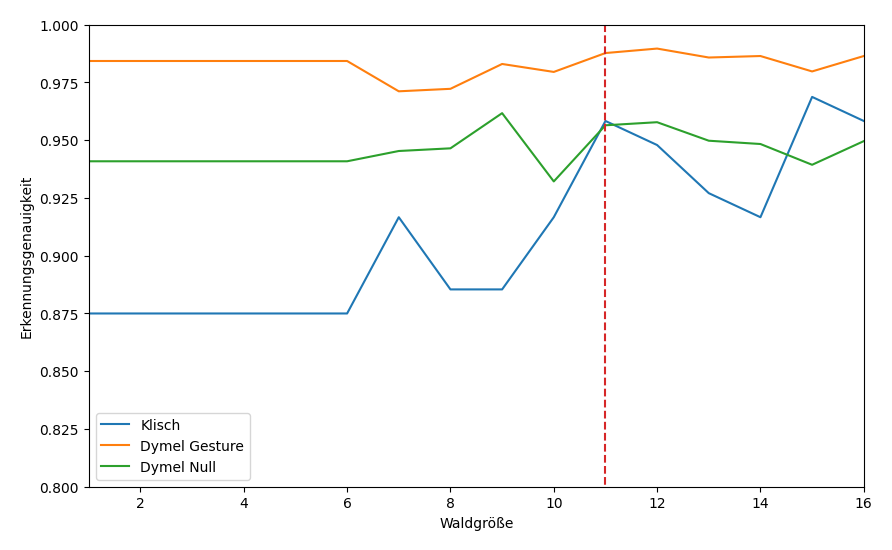
\includegraphics[width=\linewidth]{images/cocd_int_acc_per_size.png}
    \caption{Die besten Modelle pro Waldgröße der Feature-Menge Schwerpunktverteilung mit Ganzzahlen.}
    \label{fig:cocd_int_per_forest_size}
\end{figure}
Die Feature-Menge Schwerpunktverteilung mit Ganzzahlen folgt der Definition aus Kapitel \ref{sec:schwerpunktverteilung} und beinhaltet insgesamt zehn Einträge. Jeweils zwei Einträge bilden die
X- und Y-Koordinate des Schwerpunktes. Damit spiegeln zehn Einträge insgesamt fünf Zeitfenster wieder.
\newline
\newline
Aus der Tabelle \ref{tab:schwerpunktverteilung_int} sind die besten Konfigurationen jeder Kategorie zu entnehmen. Die beste Konfiguration wurde mit der Ensemble-Methode ExtraTrees gefunden.
Mit einer Klassifizierungsgenauigkeit von 95,8\% auf der Testmenge von Klisch ist dieser Ansatz nur 3,2\% schlechter als das neuronale Netz von Giese \cite{gieseThesis}. Es wurde aber auch eine Konfiguration
gefunden, wo das Modell 96,9\% der Testmenge von Klisch korrekt klassifiziert und damit nur 2,1\% schlechter ist. Diese maximiert aber in keiner Kategorie die Gesamtklassifizierungsgenauigkeit.
Außerdem werden 98,8\% der Gestentestmenge und 95,6\% der Nullgestentestmenge korrekt klassifiziert. Es wurde kein Entscheidungswald gefunden, der weniger als 44~kB Programmspeicher benötigt und besser ist als die
Konfiguration in der Kategorie \textit{Unter 28~kB}.
\newline
\newline
Der Ansatz mit Ganzzahlen erzielte eine 2,1\% höhere Gesamtklassifizierungsgenauigkeit als der Ansatz mit Gleitkommazahlen. Der 16-Bit Integer Datentyp erlaubt der Schwerpunktverteilung mit Ganzzahlen unter jeder
Restriktion größere Entscheidungswälder zu bilden, als die Schwerpunktverteilung mit Gleitkommazahlen. Abbildung \ref{fig:cocd_int_per_forest_size} zeigt einen Zuwachs der durchschnittlichen Klassifizierungsgenauigkeit
mit zunehmender Waldgröße. Es ist auszugehen, dass eine noch bessere Konfiguration gefunden werden könnte, wenn der Suchraum auf eine größere Waldgröße erweitert wird. Ähnlich wie die Schwerpunktverteilung mit
Gleitkommazahlen ist der Zuwachs der durchschnittlichen Klassifizierungsgenauigkeit ab einer Waldgröße von 7~Bäumen gering. Somit kann bereits bei einer geringen Programmgröße eine hohe Klassifizierungsgenauigkeit
erzielt werden. Damit eignet sich die Schwerpunktverteilung mit Ganzzahlen ebenfalls für kleine eingebettete Systeme.
\newline
\newline
Zu Erwarten war, dass der Ansatz mit Gleitkommazahlen bessere Ergebnisse als der Ansatz mit Ganzzahlen erzielt. Da im Training ohne Nullgestentestmenge eine besseres Modell gefunden wurde, ist davon
auszugehen, dass das equivalente Modell imt Training mit der Nullgestentestmenge nicht gefunden wurde, durch den größeren Suchraum.